\documentclass{article} 

\usepackage[utf8]{inputenc}
\usepackage{graphicx}
\usepackage[hidelinks]{hyperref} 

\renewcommand{\baselinestretch}{1.5}

\title{\Huge ADOO.\vspace{1 cm}  \\ Modelo en cascada \vspace{1 cm} }


\author{\\ \Huge Arturo Escutia López.\vspace{2 cm}\\ \Huge Profesor:Ulises Velez Saldaña}
\date{\Huge\vspace{2 cm}Septiembre 21 , 2015 \Huge  \vspace{2 cm} \\2CM12 \vspace{4 cm}}

\begin{document} 


\maketitle

 \LARGE  \textbf{Modelo de cascada }\\ \\
\large 
Se denomina modelo en cascada porque su característica principal es que no se comienza con un paso hasta que no se ha terminado el anterior. El modelo en Cascada establece que el software debe ser construido, rigurosamente, a través de una transformación sucesiva de documentos, siguiendo una estrategia lineal de desarrollo. Primero saber qué se quiere y después, cuando se conozca todo lo que se quiere, empezar a construirlo, cualquier error de diseño detectado en la etapa de prueba conduce
necesariamente al rediseño y nueva programación del código afectado, aumentando
los costos del desarrollo. \\ \\
•\textbf{Fase de ingeniería y análisis del sistema.} Debido a que el software es siempre parte de un sistema mayor el trabajo comienza estableciendo los requisitos de todos
los elementos del sistema y luego asignando algún subconjunto de estos requisitos al software.\\ \\
• \textbf{Fase de análisis de los requisitos.} Se analizan las necesidades de los
usuarios finales del software a desarrollar para determinar qué objetivos debe
cubrir. De esta fase surge una memoria llamada SRD (Documento de
Especificación de Requisitos), que contiene la especificación completa de lo
que debe hacer el sistema sin entrar en detalles internos.

 \vspace{4 cm}
• \textbf{Diseño.}El diseño del software se enfoca en cuatro atributos distintos del programa: la estructura de los datos, la arquitectura del software, el detalle procedimental y la caracterización de la interfaz. El proceso de diseño traduce los requisitos en una representación del software con la calidad requerida antes de que comience la codificación. 
\\ \\
• \textbf{Codificación.}Es la fase de programación. Aquí se desarrolla el código fuente, el diseño debe traducirse en una forma legible para la maquina. 

\begin{figure}
	\centering
	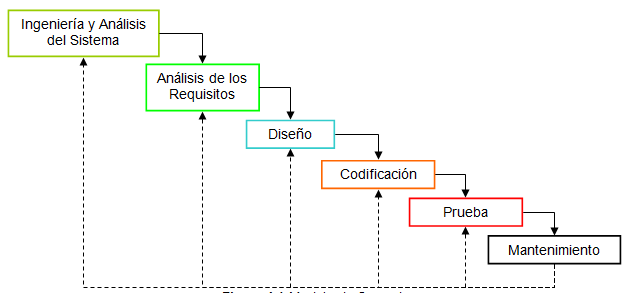
\includegraphics[width=1\linewidth, height=.4\textheight]{a}
	\caption{}
	\label{fig:a}
\end{figure}

• \textbf{Prueba.}Una vez que se ha generado el código comienza la prueba del programa. La prueba se centra en la lógica interna del software, y en las funciones externas, realizando pruebas que aseguren que la entrada definida produce los resultados que realmente se requieren. 

• \textbf{Mantenimiento.}El software sufrirá cambios después de que se entrega al cliente. Los cambios ocurrirán cuando se hayan encontrado errores, esto en lugar de que el software deba adaptarse a cambios del entorno externo


\textbf{Mantenimiento.}El software sufrirá cambios después de que se entrega al cliente. Los cambios ocurrirán cuando se hayan encontrado errores, esto en lugar de que el software deba adaptarse a cambios del entorno externo.
\\ \\

\huge \textbf {Referencias} \\ \\ 
 \large\url{-http://ciclodevidasoftware.wikispaces.com/CICLO+DE+VIDA+CASCADA+PURO}\\
\url{-http://www.ptolomeo.unam.mx:8080/xmlui/bitstream/handle/132.248.52.100/175/A5%20Cap%C3%ADtulo%202.pdf?sequence=5}\\


\end{document}
